\section{Filtro passabanda e post amplificatore}
	Per la realizzazione del filtro passabanda e del post amplificatore
	sono stati realizzati rispettivamente, impiegando le relative componentistiche, il circuito in \figurename{ \ref{fig:banda}} ed il circuito in \figurename{ \ref{fig:post}}.

	\begin{figure}[h]
		\begin{minipage}{0.75\textwidth}
			\centering
			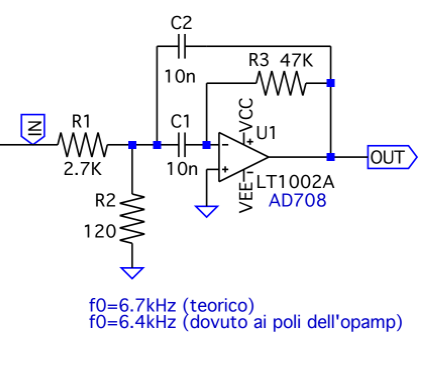
\includegraphics[scale=0.7]{banda.png}
			\caption{Filtro passabanda.}
			\label{fig:banda}
		\end{minipage}
		\begin{minipage}{0.19\textwidth}
			\begin{tabular}{l@{ }c@{ }l}
				$R_{1}$& = &\SI{2.66(3)}{\kilo\ohm}\\
				$R_{2}$& = &\SI{118(1)}{\ohm}\\
				$R_3$& = &\SI{46.4(5)}{\kilo\ohm}\\
			\end{tabular}
		\end{minipage}
	\end{figure}

	\begin{figure}[h]
		\begin{minipage}{0.75\textwidth}
			\centering
			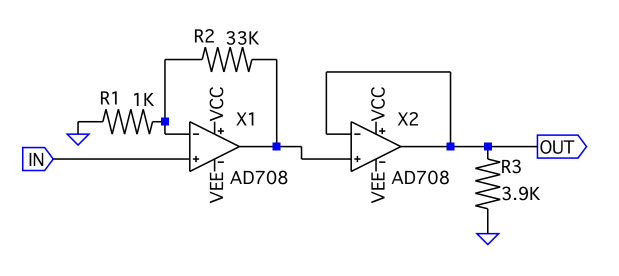
\includegraphics[width=\textwidth]{post.png}
			\caption{Post amplificatore.}
			\label{fig:post}
		\end{minipage}
		\begin{minipage}{0.19\textwidth}
			\begin{tabular}{l@{ }c@{ }l}
				$R_{1}$& = &\SI{0.972(9)}{\kilo\ohm}\\
				$R_{2}$& = &\SI{33.1(4)}{\kilo\ohm}\\
				$R_3$& = &\SI{3.87(4)}{\kilo\ohm}\\
			\end{tabular}
		\end{minipage}
	\end{figure}

	\paragraph{Verifica passa-banda}
	Per la misura della risposta in frequenza del filtro passa-banda
	è stata campionato il guadagno del circuito in risposta a dei segnali
	sinusoidali di varia frequenza. Si riportano i dati misurati nella \tab{bandp} in Appendice.

	È stato dunque eseguito un fit del guadagno, riportato in \fig{bandfit}, secondo l'equazione
	$$ A_b(\omega) = \longfrac{\alpha \omega}{\sqrt{\left(\omega^2 - \omega_0^2\right)^2 + \frac{\omega^2\omega_0^2}{Q^2}}} $$
	Ottenendo per i parametri i seguenti valori:
	$$ \alpha = \SI[per-mode=reciprocal]{32.1(2)e3}{\per\s} \qquad \omega_0 = \SI[per-mode=reciprocal]{40.29(6)e3}{\per\s} \qquad Q = \SI{9.1(3)}  \qquad \chi^2/ndof = 34/24$$
	Tali valori sono vicini a quelli attesi dai valori dei componenti utilizzati, ma se ne discostano sensibilmente, probabilmente a causa del comportamento non ideale dell'OpAmp: il centro della banda cade effettivamente a $\approx\SI{6.4}{\kHz}$ come ci si aspetta per l'effetto dei poli dell'OpAmp.

	\begin{figure}[h]
		\centering
		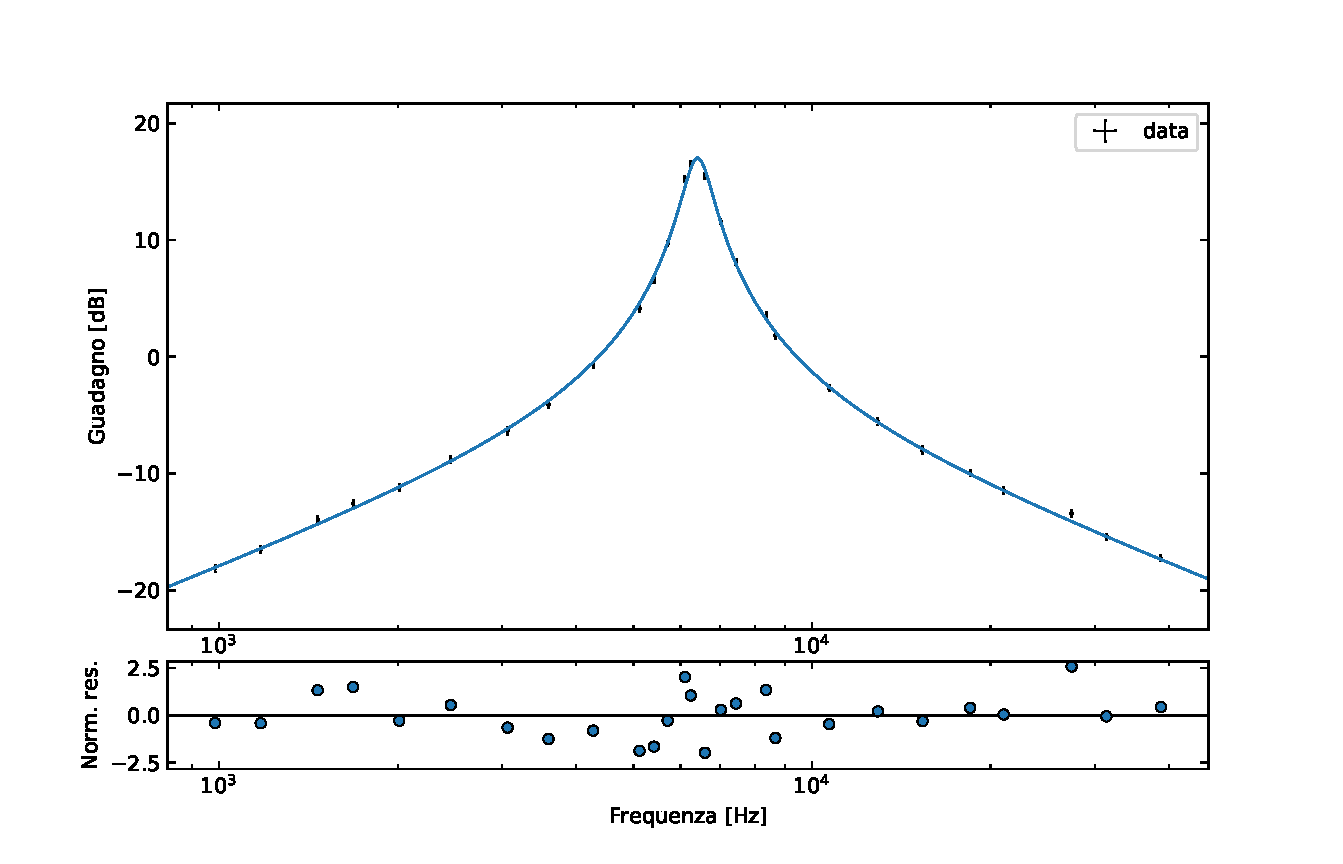
\includegraphics[scale=0.7]{fit_bandp.pdf}
		\caption{Fit del guadagno del filtro passabanda.}
		\label{fig:bandfit}
	\end{figure}

	\paragraph{Verifica post-amplificatore}
	Il circuito è costituito da un'amplificatore non invertente e da un OpAmp utilizzato come voltage follower per ridurre la resistenza in uscita di questo stadio d'amplificazione.

	Come nelle sezioni precedenti, si è misurata l'amplificazione di questo stadio separatamente dal resto del circuito, inviandogli direttamente segnali di diversa ampiezza con il generatore di forme d'onda: si è ottenuto un guadagno $A_3 = \num{34.95(2)}$, in accordo col valore atteso di $1 + \longfrac[2pt]{R_2}{R_1} = \num{35.1(4)}$.
